\documentclass[11pt]{article}
\usepackage{fullpage}
\usepackage{amsmath}
\usepackage{amssymb}
\usepackage{graphicx}
\usepackage{color}
\usepackage{float}
\usepackage{caption}
\usepackage{cases}
\usepackage{placeins}

\renewcommand\baselinestretch{1.5}
\newcommand{\Pose}{{\cal P}}
\newcommand{\A}{{\cal A}} 
\newcommand{\X}{\mathbf{X}} 
\newcommand{\symb}{\Sigma}
\newcommand{\actP}{P^{\A}}
\newcommand{\B}{\cal B}
\newcommand{\Xrm}{\X^{\Am}_{-r}}
\newcommand{\XrmPrev}{\X^{\A_{m-1}}_{-r}}
\newcommand{\Am}{\A_{m}} 
\newcommand{\Real}{\mathbb{R}}
\newcommand{\gcomp}{comp(\mathbf{g}^{\Am})}
\newcommand{\gcompPrev}{comp(\mathbf{g}^{\A_{m-1}})}
\newcommand{\qb}{\vec{q}_b}
\newcommand{\qa}{\vec{q}_a}
%\renewcommand{\prod}{\prod\limits}

\begin{document}

\title{Jeroen's model}
\maketitle

\section{Notation}

\begin{itemize}

\item $\symb$: partially-ordered list of symbols (types).

%\item $\symb_i$: ith symbol in partial ordering.

\item $T$: number of symbols in grammar.

\item $\Pose$: pose space.

\item ${\B} = (b_1,\ldots,b_N)$: set of bricks.

\item $\Pose(b) \in \Pose$: set of poses associated with brick $b$.

\item $\A = (a_1,\ldots,a_M)$, $\A \subseteq {\B}$: set of active bricks.

\item $\Am = (a_1,\ldots,a_m)$, $m \leq M$ $\Am \subseteq {\A}$: subset of active bricks.

\item $t(b)$: type of brick $b$.

\item $orph(\Am)$: the set of bricks in $\Am$ that are on ($s_a = 1$, $a \in \Am$), and are orphans (\emph{ie}, do not have a parent).

\item $\#(C)$: the cardinality (size) of some set $C$. \emph{E.g.} $\#(\A)=M$.

\item ${\cal R}$: set of production rules of the form
$A \rightarrow B_1,\ldots,B_k$ with $r = A,B_1,\ldots,B_k \in \Sigma$. ${\cal R}$ is acyclic.

\item $n(b)$: number of slots/children associated with bricks of type $t(b)$.

%\item ${\cal R}(b)$: rules with $t(b) \in \B$ in the LHS.
\item $c(b)$: the set of production rules with $t(b)$ in the LHS.

%\item $p_b$: distribution over ${\cal R}(b)$.
\item $\vec{\theta}_b \in \mathbb{R}^{\#(c(b))}$: distribution over rules with  $t(b) \in \B$ in the LHS.

%\item $p_{r,n}(x_i|x)$, $r \in {\cal R}$, $x,x_i \in {\cal P}$, $n \in [1...n(r)]$: conditional probability density over pose for $B_i$ given pose for $A$ for this rule and slot.

\item $s_b \in \{0,1\}$: on/off state of brick $b$.

\item $r_b \in {\cal R}(t(b))$: rule used by brick $b$.

\item $\mathbf{g_b} \in ( {\B} \cup \perp )^{n(b)}$: array of pointers, where each element can either point to a brick, or null (no child).

\item $\vec{q}_b \in \{\Pose(b), \perp\}$: pose for brick $b$. $\vec{q}_b = \perp$ is a ``nothing'' pose that does not contribute to image evidence.

\item $\mathbf{q}^{\Am}$: poses for bricks $a \in \Am$.

\item $\mathbf{s^{\Am}}$: on/off state for bricks $a \in \Am$.

\item $\mathbf{r^{\Am}}$: rules for bricks $a \in \Am$.

\item $\mathbf{g}_b^{\Am} \in ( {\Am} \cup \emptyset )^{n(b)}$: array of pointers, where each element can either point to a brick in the active set defined by $\Am$, or blank (child not yet specified) denoted by $\emptyset$. Note that blank is \textbf{different} than null (no child) in that blank means ``there could be a child in this slot, but we don't know if there is or which one yet'' while null (no child) means ``there definitely isn't a child in this slot''.

\item $\gcomp$: the elements of $\mathbf{g}^{\Am}$ for which $g_{b,k}^{\Am} = \emptyset$. Note: we use ``comp'' as the identifier for this concept since these are the slots that may receive a child in the future; these are the slots to be``completed''.

\item $H^{\X_{m-1}} (\vec{g}^{\Am}_b)$: set of children that $(\vec{g}^{\Am}_b)$ points to that were orphans according to $\X_{m-1}$.

\item $V(b)$: ``before'' set of bricks, which we define as $V(b) = \{b' : t(b') < t(b) \}$ where $<$ means ``comes before in the partial ordering defined by $\symb$''.

\item $W(b)$: ``after'' set of bricks, which we define as $V(b) = \{b' : t(b') > t(b) \}$ where $>$ means ``comes after in the partial ordering defined by $\symb$''.

\item $\vec{\phi}_{b,k,r} \in \mathbb{R}^{\#(W(b))+1}$: distribution over bricks to which brick $b$'s $k$th slot points to if brick $b$ is using rule $r$. Note that brick $b$ may only point to bricks in its ``after'' set. Note that the $+1$ is present since a brick/slot may point to nothing, denoted by the symbol $\perp$. \emph{edit}: this is a bit sloppy. Each slot has a particular type, and only bricks of that type may go in this slot. The set of possibilities for each slot, in general, is a subset of the ``after'' set, and not the entire after set.

\item $\vec{\pi} \in \Real^T$: vector of mixing coefficients for the templates of each type of brick.

\item $\X = \{ \mathbf{s}, \mathbf{r}, \mathbf{g}, \mathbf{q}\}$: collection of hidden variables of model.

\item $\X^{\Am} = \{ \mathbf{s^{\Am}}, \mathbf{r^{\Am}}, \mathbf{g^{\Am}}, \mathbf{q^{\Am}} \}$: collection of hidden variables for bricks $a \in \Am$.

\item $\Xrm = \{ \mathbf{s^{\Am}}, \mathbf{r^{\Am}}, \mathbf{g^{\Am}}, \mathbf{q^{\Am}} \}$: collection of hidden variables for bricks $a \in \Am$ except the hidden variables representing rules used by the bricks.

\item $Y$: the image.

\end{itemize}

\section{Model}

\begin{figure}[htbp]
\begin{center}
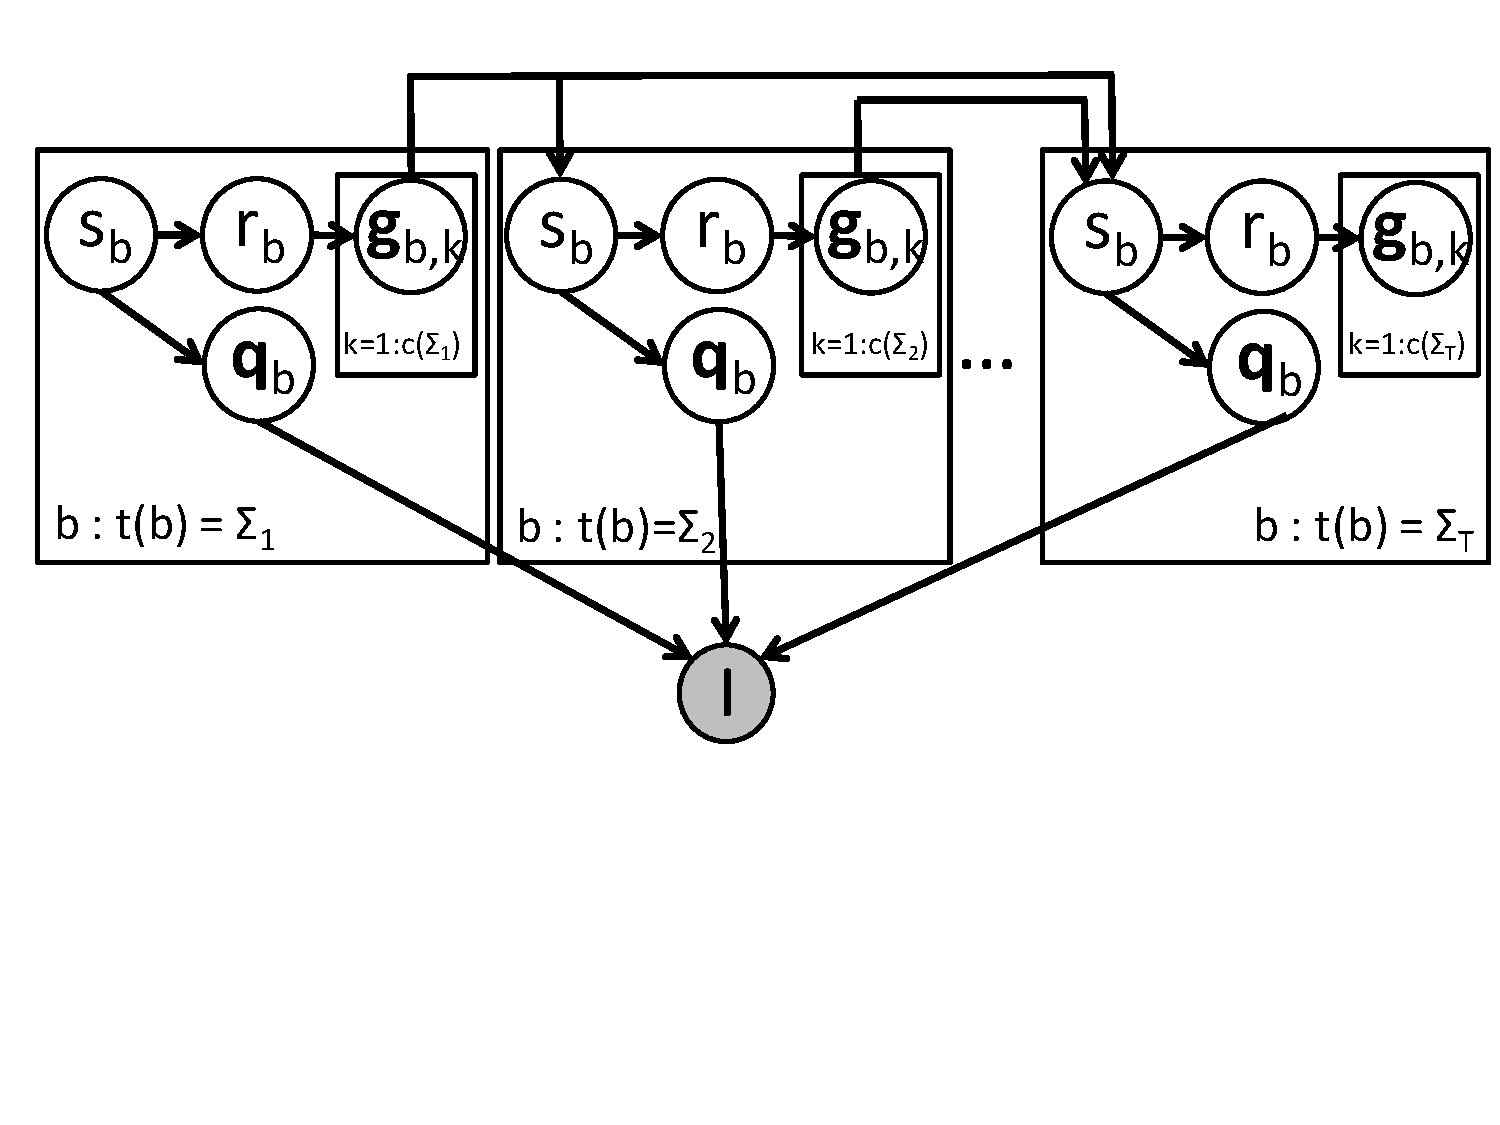
\includegraphics[width=\textwidth, trim=0cm 6cm 0cm 0cm]{gm.pdf}
\caption{Graphical model}
\label{gm}
\end{center}
\end{figure}

\FloatBarrier

The decomposition of the joint probability is given by the graphical model in Fig. \ref{gm} and by: \\

\begin{eqnarray}
P(\X, Y) &=& \big(\prod\limits_{b \in {\B}} P(s_b \mid \mathbf{g}_{V(b)}) \big ) \\
& & \times \big( \prod_{b \in {\B}} P(r_b \mid s_b) \prod_{k=1}^{n(b)} P(g_{b,k} \mid r_b) \big) \nonumber \\
& & \times \big( \prod_{b \in {\B}} P(\qb \mid s_b)\big) \nonumber \\
& & \times \big(P(Y \mid \mathbf{q}) \big) \nonumber 
\end{eqnarray}
%
where we define:
%
\begin{subnumcases}{\label{eqn.probS} P(s_b = 1 \mid \mathbf{g}_{V(b)})=} 
 1, & if $\exists$ \{a,k\} s.t. $g_{a,k} = b$ , $g_{a,k} \in {g}_{V(b)}$  \\
 \epsilon, & if $\nexists$ \{a,k\} s.t. $g_{a,k} = b$ , $g_{a,k} \in {g}_{V(b)}$
\end{subnumcases}
%
\begin{eqnarray}
P(r_b \mid s_b) &=& Discrete(\vec{\theta}_b) \\
P(g_{b,k} \mid r_b) &=& Discrete(\vec{\phi}_{b,k,r_b})
\end{eqnarray}
%
\begin{subnumcases}{P(\qb = \vec{q} \mid s_b)\big)}
\frac{1}{\#\Pose(b)}, & if $s_b = 1$, $\vec{q} \in \Pose(b)$ \\
0, & if $s_b = 1$ and $\vec{q} = \perp$ \\
0, & if $s_b = 0$, $\vec{q} \in \Pose(b)$ \\
1, & if $s_b = 0$ and $\vec{q} = \perp$
\end{subnumcases}
%
\begin{eqnarray}
P(Y \mid \mathbf{q}) &=& \prod_{p} P(Y_p \mid \mathbf{q}) \label{eqn.Yq} \\
P(Y_p \mid \mathbf{q}) &\propto& \sum_{b} \pi_{t(b)}P(Y_p \mid \qb) I(\text{template overlaps with pixel } p) \\
P(Y_p \mid \qb) &=& \text{defn here, with Bernoulli distribution and stuff}.
\end{eqnarray}

where $I(\cdot)$ is an indicator variable. 


\section*{Localization}

%For localization, we do not explicitly represent $\mathbf{r}$; instead we express the state configuration in terms of $\mathbf{g}_b^{\A}$ only, which implicitly specifies a set of compatible rules. Rather than selecting specific values for $\mathbf{r}$, we instead marginalize over the set of compatible rules defined by $\mathbf{g^{\A}}$ wherever  $\mathbf{r}$ is referred to.

We define localizations in terms of the components $\big( \prod_{b \in {\B}} P(s_b \mid \mathbf{g}_{V(b)}) \big )$, $\big( \prod_{b \in {\B}} P(r_b \mid s_b) \prod_{k=1}^{n(b)} P(g_{b,k} \mid r_b) \big)$, $\big( \prod_{b \in {\B}} P(\qb \mid s_b)\big)$, and $P(Y \mid \mathbf{q})$ separately.

\begin{eqnarray}
\big(\prod_{b \in {\B}} P(s_b \mid \mathbf{g}_{V(b)}) \big ) &\Rightarrow& \big(\prod_{a \in {\Am}} P(s_a \mid \mathbf{g}^{\Am}_{V({b})}) \big )
\end{eqnarray}

where $\Rightarrow$ is used to mean ``localiizes to''. Similarily, 

\begin{eqnarray}
\big( \prod_{b \in {\B}} P(r_b \mid s_b) \prod_{k=1}^{n(b)} P(g_{b,k} \mid r_b) \big) &\Rightarrow& \big( \prod_{a \in \Am} P(r_a \mid s_a) \prod_{k=1}^{n(a)} P^{\Am}(g_{a,k} \mid r_a) \big) \\
%
P^{\Am}(g_{a,k} \mid r_a) &=& \begin{cases} \label{actPg} 1-\sum_{a' \in {\Am}} P(g_{a,k} = a' \mid r_a) \mbox{ if } g_{a,k} = \emptyset \\
 P(g_{a,k} \mid r_a) \mbox{ , otherwise } \end{cases}
\end{eqnarray}

\begin{eqnarray}
\big( \prod_{b \in {\B}} P(\qb \mid s_b)\big) \Rightarrow \big( \prod_{a \in {\Am}} P(\qa \mid s_a)\big)
\end{eqnarray}
\begin{eqnarray}
P(Y \mid \mathbf{q}) \Rightarrow P^{\Am}(Y \mid \mathbf{q^{\Am}})
\end{eqnarray}

where we evaluate $P^{\Am}(Y \mid \mathbf{q^{\Am}})$ in a similar fashion to $P(Y \mid \mathbf{q})$ outlined in Eqn. \ref{eqn.Yq}. We note that $P^{\Am}(Y \mid \mathbf{q^{\Am}}) \neq P(Y \mid \mathbf{q^{\Am}})$ since we do not perform the correct marginalizations.

We define the overall localized distribution, $P^{\Am}(X^{\Am}$, Y), in terms of the previously defined localization distributions:
\begin{eqnarray}
P^{\Am}(X^{\Am}, Y)
&=& \big(\prod_{a \in {\Am}} P^{\Am}(s_a \mid \mathbf{g}^{\Am}_{V({b})}) \big ) \label{eqn.localJoint}\\
& & \times \big( \prod_{a \in {\Am}} P(r_a \mid s_a) \prod_{k=1}^{n(a)} P^{\Am}(g_{a,k} \mid r_a) \big) \nonumber \\
& & \times \prod_{a \in {\Am}} P(\qa \mid s_a)\big) \nonumber \\
& & \times \big( P^{\Am}(Y \mid \mathbf{q^{\Am}}) \big) \nonumber
\end{eqnarray}

\section*{State representation}

Representing the configuration of an image for a \textbf{non-localized} model requires specifying $s_b$, $g_b$, $r_b$, $\qb$, $\forall b \in \B$. For a \textbf{localized} model, the same random variables could be used as the state representation (but with $\mathbf{g^{\Am}}$ defined over a different domain than $\mathbf{g}$). However, requiring specification of the $r_b$'s is unnecessary and too restrictive; we may not be able to well predict the rule a brick has used by examining the set of active bricks. This is especially true if the active set only contains one brick! Instead, we represent the state representation of the localized model by the random variables $\Xrm = \{s_a$, $g_a$, $\qa\}$, $\forall a \in \Am$, and we marginalize over $r_a$ wherever it is used. In particular

\begin{eqnarray}
P^{\Am}(\Xrm, Y) &=& \sum_{\mathbf{r}} P^{\Am}(\X^{\Am}, Y)  \\
&=& \big( \prod_{a \in {\Am}} P^{\Am}(s_a \mid \mathbf{g}^{\Am}_{V({b})}) \big ) \label{eqn.localJointXrm} \\
& & \times \big( \prod_{a \in {\Am}} \sum_{r_a} \big(P(r_a \mid s_a) {\displaystyle \prod_{k=1}^{n(a)}} P^{\Am}(g_{a,k} \mid r_a) \big) \big) \nonumber \\
& & \times \prod_{a \in {\Am}} P(\qa \mid s_a) \nonumber \\
& & \times \big( P^{\Am}(Y \mid \mathbf{q^{\Am}}) \big). \nonumber
\end{eqnarray}

\section*{Inference}

Inference proceeds by iteratively adding one brick at a time to the active set. At any iteration, $m$, our goal is to maintain a representation of the localized posterior distribution $P^{\Am}(\Xrm \mid Y)$. To maintain this representation, we employ a particle filtering approach. We treat samples from the previous localized posterior distribution $P^{\A_{m-1}}(\X^{\A_{m-1}}_{-r} \mid Y)$ as draws from a proposal distribution, and re-weight these particles accordingly (discuss re-weighting and evaluating marginals later). Note that $P^{\A_{m-1}}(\X^{\A_{m-1}}_{-r} \mid Y) \neq P^{\A_{m}}(\X^{\A_{m-1}}_{-r} \mid Y)$; the model defined by $P^{\A_{m}}$ is different than the one defined by $P^{\A_{m-1}}$.

Suppose we have sampled a previous state $\X^{\A_{m-1}}_{-r}$, and suppose the brick we are adding to the active set is denoted $b$. To generate $\Xrm$, we need to draw values for the set of random variables defined by $\Xrm \setminus \X^{\A_{m-1}}_{-r} = \{s_b$, $\qb$, $\mathbf{g^{\Am}_b}$, $comp(g^{\A_{m-1}})\}$. That is, we need to ``expand'' the representation of $\X^{\A_{m-1}}_{-r}$ to include brick $b$. As such, we need to draw a sample from $P^{\Am}(s_b, \qb, \mathbf{g^{\Am}_b}, comp(g^{\A_{m-1}}) \mid \X^{\A_{m-1}}_{-r}, Y)$. We note that for $g \in \gcomp$, the only possible values that can be sampled for $g$ are $g = \emptyset$, $g= b$. That is, each not-yet-assigned brick slot can choose either to point to the newly-added active brick $b$, or remain empty. Note that
\begin{eqnarray}
	P^{\Am}(s_b, \qb, \mathbf{g^{\Am}_b}, comp(g^{\A_{m-1}}) \mid \X^{\A_{m-1}}_{-r}, Y) &=& \frac{P^{\Am}(s_b, \qb, \mathbf{g^{\Am}_b}, comp(g^{\A_{m-1}}), \X^{\A_{m-1}}_{-r} \mid Y)}{\sum_{s_b} \sum_{g_b}\sum_{\mathbf{g^{\Am}_b}}\sum_{comp(g^{\A_{m-1}})} P^{\Am}(s_b, \qb, \mathbf{g^{\Am}_b}, comp(g^{\A_{m-1}}), \X^{\A_{m-1}}_{-r} \mid Y)} \label{eqn.localPost1} \\
P^{\Am}(s_b, \qb, \mathbf{g^{\Am}_b}, comp(g^{\A_{m-1}}), \X^{\A_{m-1}}_{-r} \mid Y) &=& P^{\Am}(\Xrm \mid Y) \\
&\propto& P^{\Am}(\Xrm, Y). \label{eqn.localPost}
\end{eqnarray}

We first note that for any setting of the random variables outlined above, we may classify it as one of three events: 1) brick $b$ is off, 2) brick $b$ is on, and has no parents, and 3) brick $b$ is on, and has at least one parent. We compute the mass associated with each of these three events, with approximations where needed. We will be able to evaluate the denominator in Eqn. \ref{eqn.localPost1} by summing the probability mass associated with these three events. We examine these events in more detail below.

\subsection*{Event 1: brick $b$ is off}

For this event, there is only one setting of the random variables $\{s_b, \qb, \vec{g}^{\Am}_b, comp(g^{\A_{m-1}}\}$ that has non-zero probability: $s_b = 0$, $\qb = \perp$, $g_{b,k} = \perp \forall k$, $g = \emptyset$ $\forall g \in \gcompPrev$. Note that $g^{\A_{m}} \neq g^{\A_{m-1}}$ only because $g^{\A_{m-1}}$ specifies the (lack of) children for the brick $b$, which is not specified in $g^{\A_{m-1}}$. The other corresponding entries of $g^{\A_{m}}$ and $g^{\A_{m-1}}$ are indeed equal, however. It is trivial to evaluate Eqn. \ref{eqn.localJointXrm} given a particular sampled previous state, $\X^{\A_{m-1}}_{-r}$.

\subsection*{Event 1: brick $b$ is on and has no parents}

There are many settings of the random variables $\{s_b, \qb, \mathbf{g^{\Am}_b}, comp(g^{\A_{m-1}})\}$ that fall under this event. They can be characterized as: $s_b=1$, $\qb \neq \perp$ (or equivalently, $\qb \in P(b)$), $g = \emptyset$ $\forall g \in \gcompPrev$, and $g^{\Am}_{b,k} = \{\emptyset, a \text{ s.t. } a \in {\Am}\}$, $\forall k$. So, the probability mass associated with this event is given by
\begin{eqnarray}
\sum_{\vec{q}_b \in P(b)} \sum_{\vec{g}^{\Am}_{b}} P^{\Am}(s_b=1, \vec{q}_b, \vec{g}^{\Am}_{b} \gcompPrev = \emptyset, \XrmPrev, Y)
\end{eqnarray}

where we have used $\gcompPrev = \emptyset$ as a shorthand for $g = \emptyset$ $\forall g \in \gcompPrev$. Expanding, we get

\begin{eqnarray}
% \sum_{\vec{q}_b \neq \perp} \sum_{\vec{g}^{\Am}_{b}} P^{\Am}(s_b=1, \vec{q}_b, \vec{g}^{\Am}_{b} \gcompPrev = \emptyset, \X^{\A_{m-1}}, I)  \nonumber \\
&=& \sum_{\vec{g}^{\Am}_{b}} \big( \prod_{a \in {\Am}} P^{\Am}(s_a \mid \mathbf{g}^{\Am}_{V({b})}) \big ) \big( \prod_{a \in {\A_{m}}} \sum_{r_a} \big(P(r_a \mid s_a) \prod_{k=1}^{n(a)} P^{\Am}(g_{a,k} \mid r_a) \big) \big) \label{eqn.child} \\
%
& & \big( \prod_{a \in {\A_{m-1}}} P(\qa \mid s_a)\big) \big( \sum_{\vec{q}_b \in P(b)} P(\qb \mid s_b = 1)\big) P^{\Am}(Y \mid \mathbf{q^{\A_{m-1}}}, \vec{q}_b) \big). \nonumber
\end{eqnarray}

The second term in Eqn. \ref{eqn.child}, $\big( \prod_{a \in {\A_{m-1}}} P(\qa \mid s_a)\big) \big( \sum_{\vec{q}_b \in P(b)} P(\qb \mid s_b = 1)\big) P^{\Am}(Y \mid \mathbf{q^{\A_{m-1}}}, \vec{q}_b) \big)$, can be evaluated by enumerating all possible values for $\vec{q}_b \in P(b)$. In practice, whether this is practical or not is dependent on $\#(P(b))$. If $\#(P(b))$ is ``small enough'', then $\big( \prod_{a \in {\A_{m-1}}} P(\qa \mid s_a)\big) \big( \sum_{\vec{q}_b \neq \perp} P(\qb \mid s_b = 1)\big) P^{\Am}(Y \mid \mathbf{q^{\A_{m-1}}}, \vec{q}_b) \big)$ can be computed. 

Turning our attention to the first term in Eqn. \ref{eqn.child}, we note that it is not possible to efficiently compute this quantity (explain why- each slot can have $\#(Am)$ possibilities, and needs to be enumerated for each of the possible rules $b$ can take. So, this term is exponential in $\#(\Am)$. This term can be decomposed into events stating how many unique children are pointed to, but this still requires lots of computation). So we come up with approximations for it.

From the definition given in Eqn. \ref{eqn.probS}, 
%
\begin{eqnarray}
\prod_{a \in {\Am}} P^{\Am}(s_a \mid \mathbf{g}^{\Am}_{V({b})}) = \epsilon^{\#(orph(\Am))}. \label{eqn.orphan}
\end{eqnarray}
%
So to evaluate $\prod_{a \in {\Am}} P^{\Am}(s_a \mid \mathbf{g}^{\Am}_{V({b})})$ it is only necessary to find the number of orphan bricks in $\Am$.
%
Next, derive a relation between $\#(orph(\A_{m-1}))$ and $\#(orph(\A_{m}))$. If $s_b=1$ and brick $b$ does not have parents, then the number of orphans increases by $1$ since $b$ itself is an orphan. If we denote the \textbf{set} of children of $b$ given a particular $\vec{g}_b^{\Am}$ as $ch(\vec{g}_b^{\Am})$, then the number of orphans is decreased by $\#(ch(\vec{g}_b^{\Am}) \cap (orph(\A_{m-1}))$ due to $b$'s becoming the parent of these previously-orphaned bricks, and $b$ being unable to be its own child. The relation between $\#(orph(\A_{m}))$ and $\#(orph(\A_{m-1}))$ can thus be summarized as
%
\begin{eqnarray}
\#(orph(\Am)) &=& \#(orph(\A_{m-1})) + I(\text{b is orphan}) - \#(ch(\vec{g}_b^{\Am}) \cap (orph(\A_{m-1})) \\
%
&=& \#(orph(\A_{m-1})) + I(\text{b is orphan}) - \#(H^{\X_{m-1}}(\vec{g}_b^{\Am})) \label{eqn.orphanM1}
\end{eqnarray}
%
Combining Eqn. \ref{eqn.orphanM1} with Eqn. \ref{eqn.orphan} yields

\begin{eqnarray}
\prod_{a \in {\Am}} P^{\Am}(s_a \mid \mathbf{g}^{\Am}_{V({b})}) &=& \epsilon^{\#(orph(\Am))} \\
%
&=&\epsilon^{\#(orph(\A_{m-1})) + I(\text{b is orphan}) - \#(H^{\X_{m-1}}(\vec{g}_b^{\Am}))} \\
%
&=& \epsilon^{\#(orph(\A_{m-1})) + I(\text{b is orphan})} \times \epsilon^{- \#(H^{\X_{m-1}}(\vec{g}_b^{\Am}))} \label{eqn.orphan2}.
\end{eqnarray}
%
Combining Eqn. \ref{eqn.orphan2} and the first term of Eqn. \ref{eqn.child}, and noting for this event that $ I(\text{b is orphan})=1$ yields
\begin{eqnarray}
& &\sum_{\vec{g}^{\Am}_{b}} \big( \prod_{a \in {\Am}} P^{\Am}(s_a \mid \mathbf{g}^{\Am}_{V({b})}) \big ) \big( \prod_{a \in {\A_{m}}} \sum_{r_a} \big(P(r_a \mid s_a) \prod_{k=1}^{n(a)} P^{\Am}(g_{a,k} \mid r_a) \big) \big) \\
%
&=& \sum_{\vec{g}^{\Am}_{b}} \big(\epsilon^{\#(orph(\A_{m-1})) + I(\text{b is orphan})} \times \epsilon^{- \#(H^{\X_{m-1}}(\vec{g}_b^{\Am}))} \big)  \big( \prod_{a \in {\A_{m}}} \sum_{r_a} \big(P(r_a \mid s_a) \prod_{k=1}^{n(a)} P^{\Am}(g_{a,k} \mid r_a) \big) \big) \\
%
&=& \epsilon^{\#(orph(\A_{m-1})) + 1} \times \sum_{\vec{g}^{\Am}_{b}} \big( \epsilon^{- \#(H^{\X_{m-1}}(\vec{g}_b^{\Am}))} \big)  \big( \prod_{a \in {\A_{m}}} \sum_{r_a} \big(P(r_a \mid s_a) \prod_{k=1}^{n(a)} P^{\Am}(g_{a,k} \mid r_a) \big) \big) \\
%
&=& \epsilon^{\#(orph(\A_{m-1})) + 1} \big( \prod_{a \in {\A_{m}}, a \neq b} \sum_{r_a} \big(P(r_a \mid s_a) \prod_{k=1}^{n(a)} P^{\Am}(g_{a,k} \mid r_a) \big) \big) \label{bottomup} \\
& & \times \sum_{\vec{g}^{\Am}_{b}} \big( \epsilon^{- \#(H^{\X_{m-1}}(\vec{g}_b^{\Am}))} \big) \big( \sum_{r_b} \big(P(r_b \mid s_b = 1) \prod_{k=1}^{n(b)} P^{\Am}(g_{b,k} \mid r_b) \big) \nonumber \\
%
&=& \epsilon^{\#(orph(\A_{m-1})) + 1} \big( \prod_{a \in {\A_{m}}, a \neq b} \sum_{r_a} \big(P(r_a \mid s_a) \prod_{k=1}^{n(a)} P^{\Am}(g_{a,k} \mid r_a) \big) \big) \\
& & \times E<\epsilon^{- \#(H^{\X_{m-1}}(\vec{g}_b^{\Am}))}>_{P(\vec{g}^{\Am}_{b} \mid s_b = 1)} \nonumber
\end{eqnarray}

where $E<\cdot>_{P(x)}$ denotes an expectation under the distribution $P(x)$, and $P(\vec{g}^{\Am}_{b} \mid s_b = 1) = \sum_{r_b} P(r_b \mid s_b = 1) \prod_{k=1}^{n(b)} P^{\Am}(g_{b,k} \mid r_b)$. Note that $P(\vec{g}^{\Am}_{b} \mid s_b = 1) \neq \prod_{k=1}^{n(b)} P(g_{b,k} \mid s_b=1)$. This can be seen by examining the graphical model in Fig. \ref{gm} and noting that if $r_b$ is unobserved (marginalized over), then the paths between the $g_{b,k}$'s is not blocked. This is the source of our inability to compute the probability mass associated with this event exactly. Each of the $g_{b,k}$ slots has $\#(\Am)$ possibilities, and so exact inference would require enumerating all of the $\#(\Am)^{n(b)+1}$ possibilities for $\vec{g}_{b}$ for each of the $\#(c(b))$ possible rules. We outline two strategies for dealing with the intractability: For coming child approximations, do both slot-centric view (Pedro's approximation) and child-centric view (Jeroen's approximation)


%\begin{figure}[htbp]
%\begin{center}
%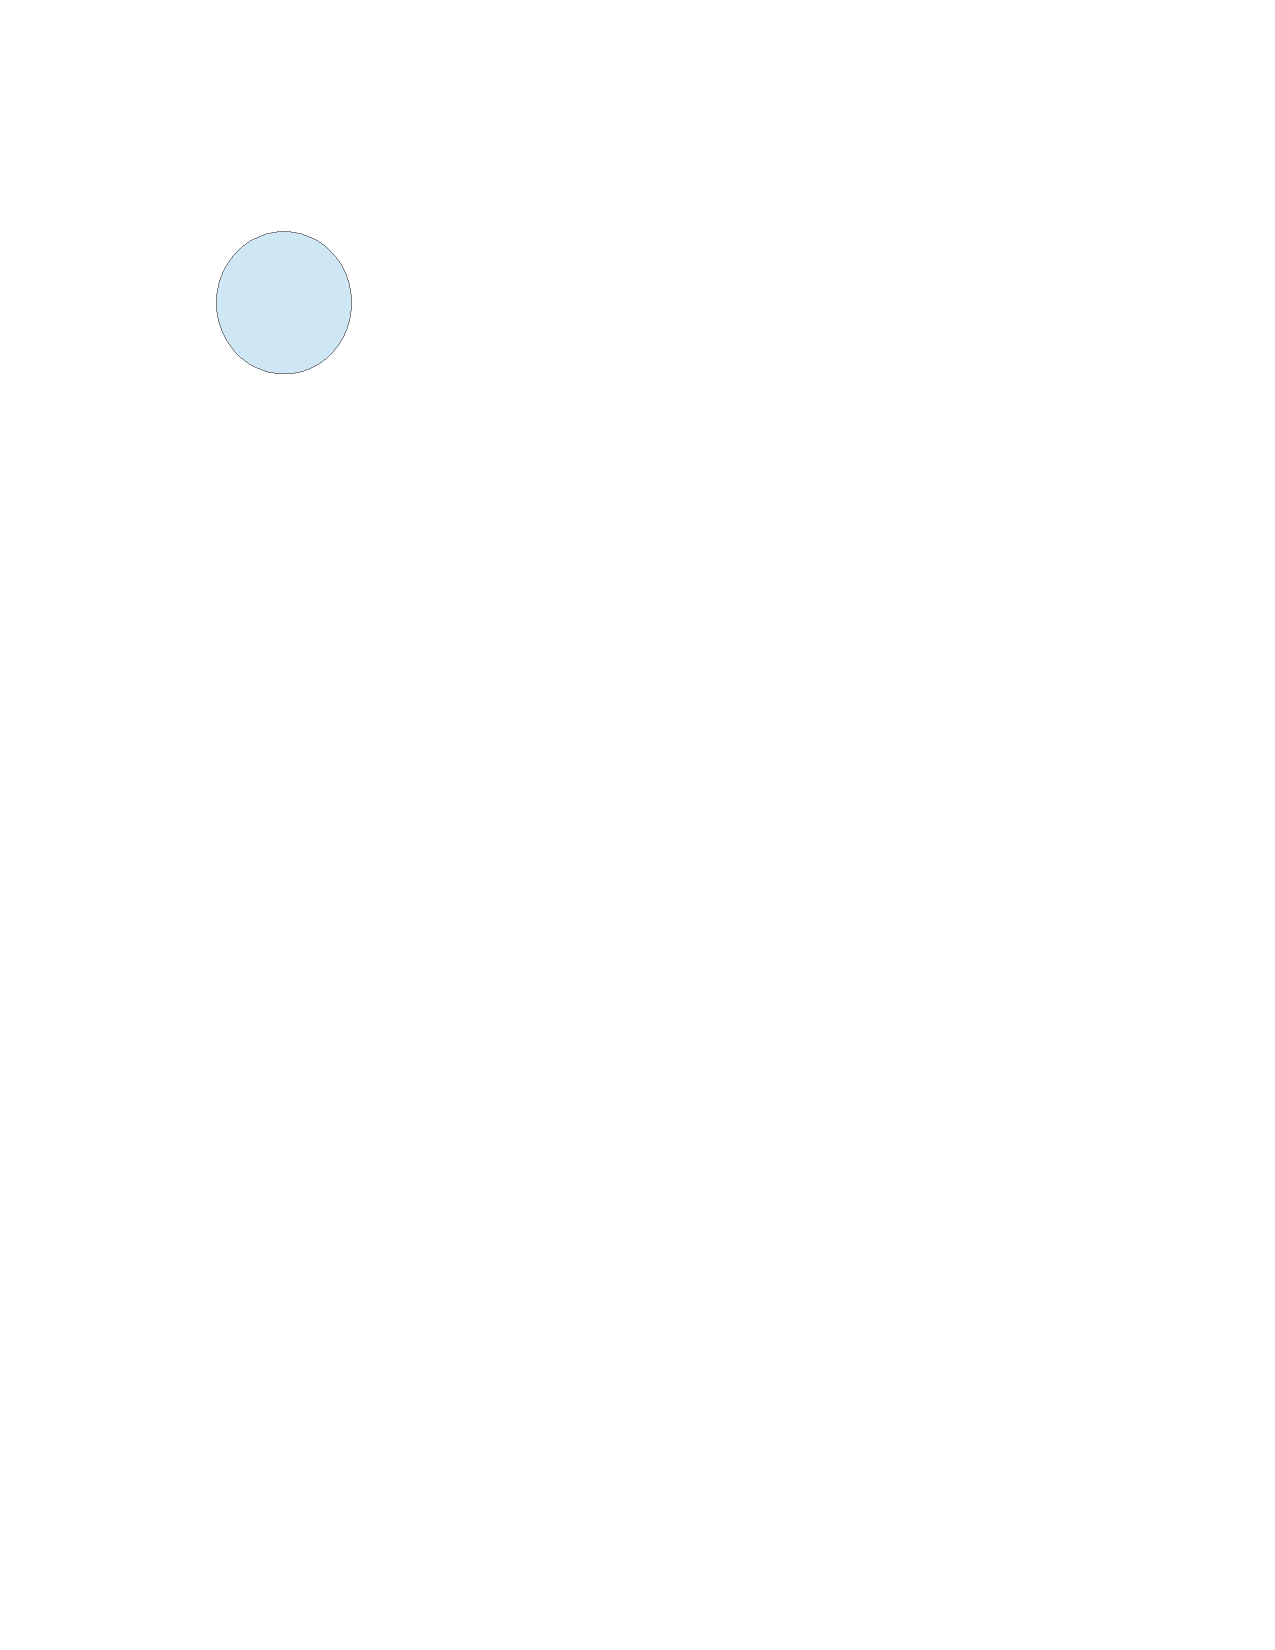
\includegraphics[width=\textwidth]{test.pdf}
%\caption{Graphical model}
%\end{center}
%\end{figure}


\end{document}
